% !TeX program = xelatex
% AES v0.1. Start here; replace the sample text with your paper.
% Overleaf: select XeLaTeX in project settings, then compile main.tex.
% Local: latexmk -xelatex main.tex
\documentclass[11pt,a4paper]{article}
\usepackage{aes} % Public. For anonymous review, use \usepackage[review]{aes}.

% Optional packages used by this example.
\usepackage{amsmath,tabularx}

% Optional short title in brackets; full title in braces.
\title[Your Short Paper Title]{Your Paper Title}

% affil: institution IDs; equal: joint contribution; corresponding: contact author.
\aesauthor[affil={1},equal,corresponding]{Author One}
\aesauthor[affil={1,2},equal]{Author Two}
\aesauthor[affil={2}]{Author Three}
\aesaffiliation{1}{Institution A}
\aesaffiliation{2}{Institution B}

% Use raw email addresses; do not escape _ or @. Delete this line to omit emails.
\aesemails{\aesemail{author_one@example.org}\quad\aesemail{author_two@example.org}}

% Optional metadata and author notes. Remove the leading % to enable.
% \aeskeywords{Agent evaluation; Benchmarking; Reliability}
% \aesequalnote{These authors contributed equally.}
% \aescorrespondingnote{Correspondence to Author One.}

\begin{document}
\maketitle

\begin{abstract}
Replace this abstract with a concise account of the research question, approach,
main findings, and limitations. Explain what is evaluated and why the evidence
supports the central claim. Define any essential terms and keep the abstract
self-contained. This sample demonstrates the Agent Evaluation Science template,
including author information, citations, figures, tables, equations, footnotes,
and appendices. All numerical results below are invented for illustration.
\end{abstract}

\section{Introduction}
\label{sec:introduction}
Introduce the research problem, explain its significance, and state the paper's
contribution. Identify the system, task, or evaluation resource under study.
Describe the gap addressed by the work and distinguish it from the closest
existing approaches. The text in this document is a writing scaffold, not a
report of completed research.

% Use a blank line between paragraphs. Do not add indentation or manual \\ breaks.
A new paragraph has no first-line indentation. The template supplies paragraph
spacing, heading sizes, and page margins. Use ordinary LaTeX markup such as
\textbf{bold}, \emph{italics}, and \url{https://evalscience.org/}. Keep formatting
commands out of prose unless they communicate a meaningful distinction.
A footnote can hold a brief supporting detail.\footnote{Use footnotes for concise
qualifications or supplementary information. Keep essential evidence in the main text.}

\section{Related Work}
\label{sec:related}
% \citet: Author (year). \citep: (Author, year). Keys come from references.bib.
A narrative citation uses \citet{hua2025charting}. A parenthetical citation
uses \citep{na2025psychotherapy}. Multiple sources can share a citation
\citep{ma2025manipulation,hua2025scoping}. These real publications provide citation
examples; replace them with sources relevant to your paper.

Explain how prior approaches define their tasks, gather evidence, and assess
outcomes. Connect each cited source to a specific statement. When revisiting a
source, cite it again where needed \citep{hua2025charting}. The numbers after
``Cited at:'' in References return to individual citation occurrences, including
repeated citations on the same page; they are not page numbers.

\section{Method}
\label{sec:method}
Describe the procedure in enough detail that another researcher can understand
what was measured and reproduce the essential steps. Separate decisions about
task construction, experimental conditions, and outcome assessment. State which
parts of the procedure were fixed before examining the results.

\subsection{Evaluation Setup}
\label{sec:setup}
Specify the inputs, available tools, environment, and resource limits. For
example, an evaluation description can identify:
\begin{itemize}
  \item The tasks and the criteria used to select them.
  \item The information and tools available to each system.
  \item The conditions under which an attempt is considered complete.
\end{itemize}
Record relevant model versions and evaluation dates. Explain whether attempts
are independent and how failures, retries, and incomplete records are handled.

\subsubsection{Outcome Measures}
\label{sec:measures}
% Add a label inside the equation; refer to it with \eqref.
Let $N$ be the number of evaluated attempts and $s_i\in\{0,1\}$ indicate whether
attempt $i$ meets the stated success criteria. The completion rate is
\begin{equation}
  \widehat{S}=\frac{1}{N}\sum_{i=1}^{N}s_i.
  \label{eq:success}
\end{equation}
Define the unit of analysis and the denominator for every measure. If partial
success or abstention is possible, explain how it is represented rather than
silently removing those outcomes from Equation~\eqref{eq:success}.

\subsection{Procedure}
A numbered list is useful when order matters:
\begin{enumerate}
  \item Initialize the environment and provide the task instruction.
  \item Record actions, observations, and resource use during execution.
  \item Assess the outcome using the predefined scoring procedure.
\end{enumerate}
Figure~\ref{fig:workflow} summarizes the relationship between these stages.
Use descriptive labels and refer to figures and tables by number.

% Put captions below figures and tables, and labels after captions.
% Replace the sample PDF with your own figure. Prefer vector PDFs for diagrams.
\begin{figure}[htbp]
  \centering
  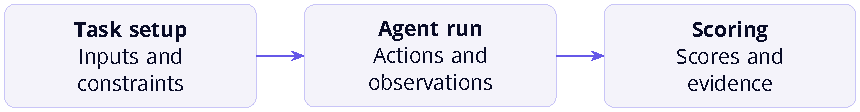
\includegraphics[width=\linewidth]{assets/example-figure.pdf}
  \caption{An illustrative evaluation workflow. Replace this diagram and caption
  with a figure that supports the paper's argument.}
  \label{fig:workflow}
\end{figure}

\section{Results and Discussion}
\label{sec:results}
Present the main findings and explain what they establish. Table~\ref{tab:results}
uses invented values to demonstrate a compact results table. State the meaning
of each column, the direction of improvement, and the evaluation conditions.
Use actual observations and suitable uncertainty estimates in a research paper.

% booktabs is already loaded by aes. Avoid vertical rules and manual scaling.
\begin{table}[htbp]
  \centering
  \begin{tabularx}{\linewidth}{@{}Xrr@{}}
    \toprule
    System & Completion (\%) & Mean actions \\
    \midrule
    Baseline & 61.0 & 14.2 \\
    Variant A & 68.5 & 12.8 \\
    Variant B & 72.0 & 13.1 \\
    \bottomrule
  \end{tabularx}
  \caption{Synthetic results for layout demonstration. Completion is the
  percentage of successful attempts; mean actions measures resource use.}
  \label{tab:results}
\end{table}

Discuss both successful and unsuccessful cases. A higher aggregate score may
hide differences in task coverage, failure modes, or resource use. Explain the
scope of the comparison and connect quantitative results to the evidence needed
to interpret them. Appendix~\ref{app:details} illustrates supplementary material.

\section{Limitations}
Describe which settings, populations, or tasks the evidence does not cover.
Explain limitations of the measurement procedure and any unresolved sources of
uncertainty. The limitations of this sample are straightforward: no experiment
was run, and the results table contains fictional values.

\section{Conclusion}
State what the work establishes and identify the most consequential remaining
question. Keep the conclusion consistent with the reported evidence. Remove all
sample prose, fictional results, and unused examples before sharing your paper.

% Optional. This entire block is omitted in review mode.
\begin{aespubliconly}
\aesbackmattersection{Acknowledgments}
Replace with acknowledgments, or delete this block.
\end{aespubliconly}

% Optional unnumbered section. This one remains visible in review mode.
\aesbackmattersection{Ethics Statement}
Describe relevant ethical considerations, or delete this section if not applicable.

% aes selects the bibliography style. Edit entries in references.bib.
\bibliography{references}

% Appendices start on a new page. Use normal sections and labels.
\appendix
\section{Additional Evaluation Details}
\label{app:details}
Place supporting protocols, additional analyses, and extended results here.
Appendix figures and tables use labels such as Figure A1 and Table A1.
Refer to the relevant appendix from the main text so that readers know why the
additional material matters.

\subsection{Reporting Details}
\begin{itemize}
  \item Provide the task selection criteria and any exclusions.
  \item Record model identifiers, tool access, and resource budgets.
  \item Describe scoring, review, and disagreement resolution.
\end{itemize}

% For tables spanning pages, use aeslongtable; see docs/USAGE.md.
\begin{table}[htbp]
  \centering
  \begin{tabularx}{\linewidth}{@{}lX@{}}
    \toprule
    Field & Description \\
    \midrule
    Task ID & Stable identifier for the evaluated task. \\
    Outcome & Success, failure, or an explicitly defined unresolved state. \\
    Evidence & The observation or record supporting the assigned outcome. \\
    \bottomrule
  \end{tabularx}
  \caption{An example reporting schema for supplementary evaluation records.}
  \label{tab:schema}
\end{table}

\end{document}
